\documentclass[12pt]{article}
\usepackage[T1]{fontenc}
\usepackage[utf8]{inputenc}
\usepackage[fleqn]{amsmath}
\usepackage{tikz}
\usetikzlibrary{arrows.meta}
\usetikzlibrary{calc}
\usetikzlibrary{ decorations.markings}
\usetikzlibrary{positioning}

\begin{document}

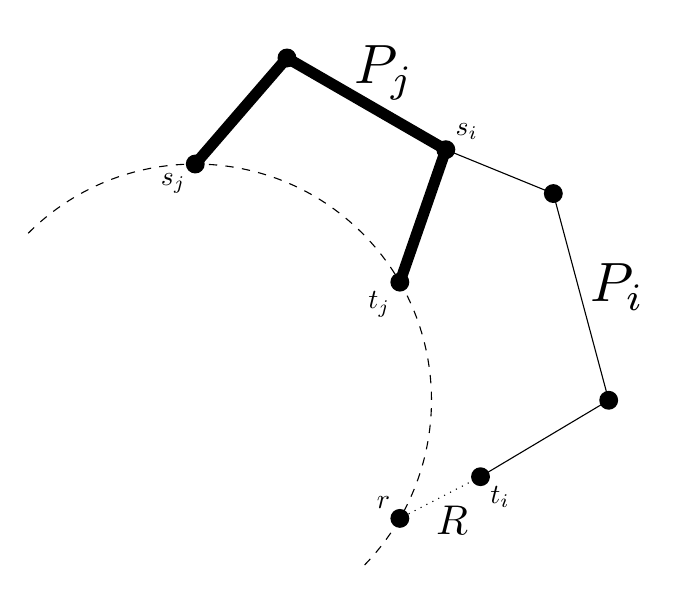
\begin{tikzpicture}[scale=1.5]
				\draw[dashed] (135:2) arc (135:-45:2);
				
				\coordinate (V11) at (90:2);
				\coordinate (V12) at (75:3);
				\coordinate (V13) at (45:3);
				\coordinate (V14) at (30:2);
				
				\node[above right] at (V13) {$s_i$};
				\node[below left] at (V14) {$t_j$};
				\node[below left] at (V11) {$s_j$};
				\node[scale=2] at(60:3.2) {$P_j$};
				
				\foreach \i in {1, 2, 3, 4}
				{
					\path[fill=black] (V1\i) circle (0.08);
				}
				
				\foreach \i/\j in {1/2, 2/3, 3/4}
				{
					\path[draw][line width=4pt](V1\i) -- (V1\j);
				}
				
				\coordinate (V21) at (30:3.5);
				\coordinate (V22) at (0:3.5);
				\coordinate (V23) at (-15:2.5);
				\coordinate (V24) at (-30:2);
				
				\node[below right] at (V23) {$t_i$};
				\node[above left] at (V24) {$r$};
				\node[scale=2] at(15:3.7) {$P_i$};
				\node[scale=1.5] at(-25:2.4) {$R$};
				
				\foreach \i in {1, 2, 3, 4}
				{
					\path[fill=black] (V2\i) circle (0.08);
				}
				
				\foreach \i/\j in {1/2, 2/3}
				{
					\path[draw](V2\i) -- (V2\j);
				}
				\path[draw](V13) -- (V21);
				\path[draw][dotted](V23) -- (V24);
			\end{tikzpicture}

\end{document}